\documentclass[border=5pt]{standalone}
\usepackage{tikz}
\usepackage[T1]{fontenc}
\usepackage{helvet}
\renewcommand{\familydefault}{\sfdefault}
\usetikzlibrary{arrows.meta, positioning}

\begin{document}
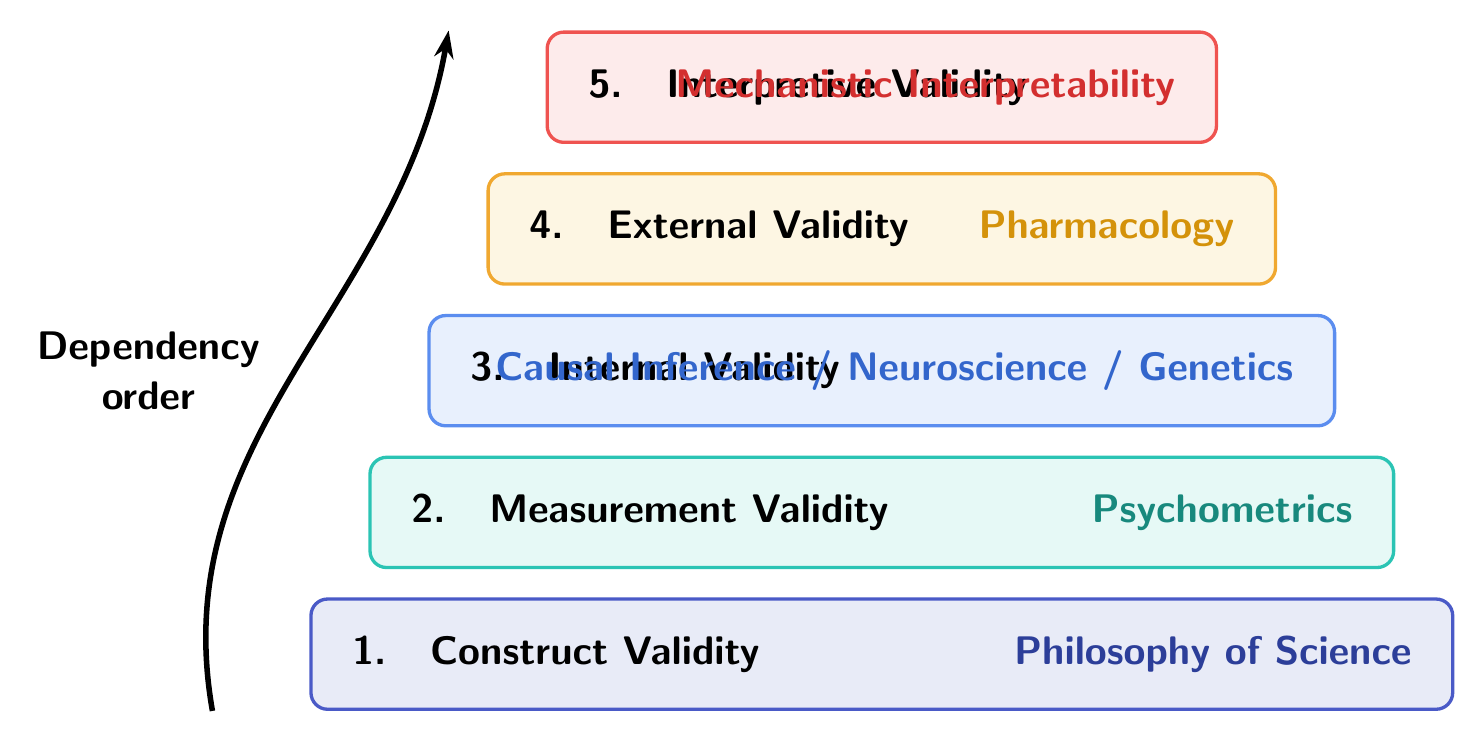
\begin{tikzpicture}[
    every node/.style={font=\sffamily},
    layer/.style={
        minimum height=1.4cm,
        rounded corners=6pt,
        draw,
        line width=1.2pt,
        text depth=0pt,
    }
]

% Colors matching the original
\definecolor{bluepurple}{HTML}{4A5AC7}
\definecolor{tealgreen}{HTML}{2BC4B4}
\definecolor{steelblue}{HTML}{5B8DEF}
\definecolor{ambergold}{HTML}{F0A830}
\definecolor{coralred}{HTML}{EF5350}

\definecolor{fillblue}{HTML}{E8EBF7}
\definecolor{fillteal}{HTML}{E6F9F6}
\definecolor{fillsteelblue}{HTML}{E8F0FD}
\definecolor{fillyellow}{HTML}{FDF6E3}
\definecolor{fillpink}{HTML}{FDEBEB}

\definecolor{textblue}{HTML}{2C3E99}
\definecolor{textteal}{HTML}{18897D}
\definecolor{textsteelblue}{HTML}{3366CC}
\definecolor{textamber}{HTML}{D4920A}
\definecolor{textred}{HTML}{D32F2F}

% Layer widths (pyramid shape)
\def\wA{14.5cm}
\def\wB{13cm}
\def\wC{11.5cm}
\def\wD{10cm}
\def\wE{8.5cm}

% Vertical spacing
\def\vgap{1.8cm}

% Draw layers bottom to top
\node[layer, fill=fillblue, draw=bluepurple, minimum width=\wA] (L1) at (0,0) {};
\node[layer, fill=fillteal, draw=tealgreen, minimum width=\wB] (L2) at (0,\vgap) {};
\node[layer, fill=fillsteelblue, draw=steelblue, minimum width=\wC] (L3) at (0,2*\vgap) {};
\node[layer, fill=fillyellow, draw=ambergold, minimum width=\wD] (L4) at (0,3*\vgap) {};
\node[layer, fill=fillpink, draw=coralred, minimum width=\wE] (L5) at (0,4*\vgap) {};

% Layer text - left side (number + validity type)
\node[font=\sffamily\bfseries\Large, anchor=west, text=black] at ([xshift=12pt]L1.west) {\textbf{1.}\quad Construct Validity};
\node[font=\sffamily\bfseries\Large, anchor=west, text=black] at ([xshift=12pt]L2.west) {\textbf{2.}\quad Measurement Validity};
\node[font=\sffamily\bfseries\Large, anchor=west, text=black] at ([xshift=12pt]L3.west) {\textbf{3.}\quad Internal Validity};
\node[font=\sffamily\bfseries\Large, anchor=west, text=black] at ([xshift=12pt]L4.west) {\textbf{4.}\quad External Validity};
\node[font=\sffamily\bfseries\Large, anchor=west, text=black] at ([xshift=12pt]L5.west) {\textbf{5.}\quad Interpretive Validity};

% Layer text - right side (discipline)
\node[font=\sffamily\bfseries\Large, anchor=east, text=textblue] at ([xshift=-12pt]L1.east) {Philosophy of Science};
\node[font=\sffamily\bfseries\Large, anchor=east, text=textteal] at ([xshift=-12pt]L2.east) {Psychometrics};
\node[font=\sffamily\bfseries\Large, anchor=east, text=textsteelblue] at ([xshift=-12pt]L3.east) {Causal Inference / Neuroscience / Genetics};
\node[font=\sffamily\bfseries\Large, anchor=east, text=textamber] at ([xshift=-12pt]L4.east) {Pharmacology};
\node[font=\sffamily\bfseries\Large, anchor=east, text=textred] at ([xshift=-12pt]L5.east) {Mechanistic Interpretability};

% Dependency arrow on left
\draw[-{Stealth[length=10pt, width=7pt]}, line width=2pt, black]
    ([xshift=-35pt]L1.south west) to[out=100, in=260]
    node[midway, left=8pt, font=\sffamily\bfseries\Large, text=black, align=center] {Dependency\\order}
    ([xshift=-35pt]L5.north west);

\end{tikzpicture}
\end{document}
